% Created 2014-01-21 Tue 19:14
\documentclass[11pt, letterpaper, oneside, spanish]{scrbook}
	    \usepackage[spanish]{babel}

	    \usepackage{geometry}
	    \usepackage{lastpage}

	    \geometry{	
	        headsep=12mm	
	    }
 	    \usepackage{graphicx}

            \usepackage[usenames,dvipsnames]{color}
            \usepackage{titlesec}
           
%% Makeover cantv 
  
            \usepackage{xcolor}
            \usepackage{lmodern}
            \renewcommand*{\familydefault}{\sfdefault}

         
            \titleformat{\chapter}
            {\color{black}\Huge\bfseries}
            {\color{black}\Huge\bfseries\thechapter}{1em}{}
            
            \titleformat{\section}
            {\color{black}\LARGE\bfseries}
            {\color{black}\LARGE\bfseries\thesection}{1em}{}
            

            \titleformat{\subsection}
            {\color{black}\Large\bfseries}
            {\color{black}\Large\bfseries\thesubsection}{1em}{}


%% end makeover 

	    \usepackage[ilines, komastyle]{scrpage2}
	    \pagestyle{scrheadings}	     
	    \clearscrheadfoot
	    \ihead[ 
            \vspace{0cm}
            \hspace{11cm}
	     	\includegraphics{/usr/share/covetel-doc/imgs/logo-cantv} 
		]{
            \vspace{0cm}
            \hspace{11cm}
		    \includegraphics{/usr/share/covetel-doc/imgs/logo-cantv}
		}
	    \cfoot[ 
            \vspace{1.5cm}
            \hspace{0cm}
            \pagemark/\pageref{LastPage} 
         ]{ 
            \vspace{1.5cm}
            \hspace{0cm}
            \pagemark/\pageref{LastPage} 
         }
        \ifoot[ 
	        \includegraphics{/usr/share/covetel-doc/imgs/footer_cantv} 
		]{
		    \includegraphics{/usr/share/covetel-doc/imgs/footer_cantv}
		}
\usepackage[utf8]{inputenc}
\usepackage[T1]{fontenc}
\usepackage{fixltx2e}
\usepackage{graphicx}
\usepackage{longtable}
\usepackage{float}
\usepackage{wrapfig}
\usepackage{soul}
\usepackage{textcomp}
\usepackage{marvosym}
\usepackage{wasysym}
\usepackage{latexsym}
\usepackage{amssymb}
\usepackage{hyperref}
\tolerance=1000
\usepackage{array}
\renewcommand\maketitle{
    \begin{titlepage}
      \begin{center}
        \includegraphics{/usr/share/covetel-doc/imgs/covetel2} 
        \\[1cm]
        {
          \Huge
          \color{Black}
          \fontseries{sbc}\selectfont
        }
        \\[1cm]
        {
          \huge
          \color{Gray}
          \fontseries{sbc}\selectfont
          Análisis de Brecha Portal cantv.com.ve
        }
        \\[1cm]
          {
            \huge
            \color{covetelred}
            \fontseries{sbc}\selectfont
            CANTV
        \\[1cm]
            Enero, 2014
          }
      \end{center}
      \begin{flushleft}

          \vspace{1cm} \footnotesize \hspace{10cm} \color{Gray} RIF:
          J-29532381-6
                                                                                                                                                      
      \smallskip

      \hspace{10cm} \color{Gray} Contacto: 

      \smallskip
    
      \hspace{10cm} \color{Gray} 0276-3556899 
    
      \smallskip
    
      \hspace{10cm} \color{Gray} 0416-5023759 
    
      \smallskip
    
      \hspace{10cm} \color{Gray} info@covetel.com.ve

      \end{flushleft}


    \end{titlepage}
}

\providecommand{\alert}[1]{\textbf{#1}}

\title{Análisis de brecha Portal cantv.com.ve}
\author{Carlos Paredes}
\date{2014-1-16}
\hypersetup{
  pdfkeywords={},
  pdfsubject={Análisis de brecha Portal cantv.com.ve},
  pdfcreator={Emacs Org-mode version 7.9.3f}}

\begin{document}

\maketitle

\setcounter{tocdepth}{3}
\tableofcontents
\vspace*{1cm}

\chapter{Versiones del Documento}
\label{sec-1}


\includegraphics[width=.9\linewidth]{images/versiones_brecha_cantv_com_ve_29158ccac4c6f0e1492879c720bc2bf907805474.png}
\chapter{cantv.com.ve Requerimientos Funcionales}
\label{sec-2}
\section{Funcionalidades:}
\label{sec-2-1}
\subsection{General / Guía de Navegación}
\label{sec-2-1-1}

\begin{itemize}
\item Nombre: Breadcrumbs o guía de navegación aplicado en todo el portal
\item Prioridad: Mandatorio
\item Esfuerzo: Funcionalidad existente en Plone
\item Aplicación que cubrirá la funcionalidad:  built-in
\end{itemize}
\subsection{General / Archivos}
\label{sec-2-1-2}

\begin{itemize}
\item Nombre: El sistema debe permitir la carga de archivos de cualquier tipo,
  tales como documentos en formatos de Libre Office, Microsoft Office, PDF
  etc.
\item Prioridad: Mandatorio
\item Esfuerzo: Funcionalidad existente en Plone
\item Aplicación que cubrirá la funcionalidad:  built-in
\end{itemize}
\subsection{General / Mapa de Sitio}
\label{sec-2-1-3}

\begin{itemize}
\item Nombre: Mapa de sitio
\item Descripción: Mapa de sitio
\item Prioridad: Mandatorio
\item Esfuerzo: Funcionalidad existente en Plone
\item Aplicación que cubrirá la funcionalidad:  built-in
\end{itemize}
\subsection{General / Noticias}
\label{sec-2-1-4}

\begin{itemize}
\item Nombre: Noticias.
\item Descripción: Noticias, permite la carga de notas de prensa y posee los
  siguientes campos:
\begin{itemize}
\item Antetítulo
\item Titulo
\item Sumario
\item Contenido
\item Permite la carga de Imagen(es) interna(s)
\item Campos para la carga y enlace hacia archivos, vídeos
\item Botón de conversión a formato PDF
\item Botón imprimir contenido
\end{itemize}
\item Prioridad: Mandatorio
\item Esfuerzo: Funcionalidad existente en Plone
\item Aplicación que cubrirá la funcionalidad:  built-in
\end{itemize}
\subsection{General / Documentos}
\label{sec-2-1-5}

\begin{itemize}
\item Nombre: Documentos: permite cargar documentos en formatos de Libre Office,
  Microsoft Office, PDF etc.
\item Prioridad: Mandatorio
\item Esfuerzo: Funcionalidad existente en Plone
\item Aplicación que cubrirá la funcionalidad:  built-in
\end{itemize}
\subsection{General / Programación de contenido}
\label{sec-2-1-6}

\begin{itemize}
\item Nombre: Se debe programar el contenido
\item Prioridad: Mandatorio
\item Esfuerzo: Funcionalidad existente en Plone
\item Aplicación que cubrirá la funcionalidad:  built-in
\end{itemize}
\subsection{Administración de Contenido}
\label{sec-2-1-7}

\begin{itemize}
\item Nombre: Permisología para las UPS
\item Descripción: Las UPS solo podrán realizar la carga, actualización de
  contenido y solicitud de cambio de plantilla del minisitio, de los productos
  y servicios que estén asociados a su rol y área de competencia. La revisión
  y aprobación de los contenidos cargados por las UPS corresponde a la GGCAP.
\item Prioridad: Mandatorio
\item Esfuerzo: Funcionalidad existente en Plone, pero requiere configuración ya
  parametrización
\item Aplicación que cubrirá la funcionalidad: Roles
\end{itemize}
\subsection{RSS / Atom}
\label{sec-2-1-8}

\begin{itemize}
\item Nombre: RSS/Atom
\item Descripción: Permitir la creación de varios RSS según la taxonomía del
  portal, los minisitios, o la taxonomía definida en Sala prensa. Al hacer
  clic en el logo de RSS este ultimo deberá enlazar a una sección en donde se
  muestre el listado los RSS previamente definidos por los administradores del
  sitio.
\begin{itemize}
\item Sindicación de contenidos mediante el uso de RSS/Atom
\end{itemize}
\item Prioridad: Mandatorio
\item Esfuerzo: Funcionalidad existente en Plone, pero requiere configuración ya
  parametrización
\item Aplicación que cubrirá la funcionalidad:  built-in
\end{itemize}
\subsection{Administración de Contenido}
\label{sec-2-1-9}

\begin{itemize}
\item Nombre: La administración, carga de contenido, aplicación de la plantilla y
  publicación del portal cantv.com.ve corresponde a la Gerencia General de
  Comunicaciones y Asuntos Públicos (GGCAP).
\item Prioridad: Mandatorio
\item Esfuerzo: Funcionalidad existente en Plone, pero requiere configuración ya
  parametrización
\item Aplicación que cubrirá la funcionalidad: Roles
\end{itemize}
\subsection{General / Encuesta}
\label{sec-2-1-10}

\begin{itemize}
\item Nombre: El portal debe poseer un módulo con la capacidad de generar una
  encuesta breve, que permita o no la visualización de los resultados a los
  usuarios participantes según el criterio de los administradores. Para
  usuarios del portal , pueden ser anónimas.
\item Prioridad: Mandatorio
\item Esfuerzo: Funcionalidad existente en Plone, pero requiere configuración ya
  parametrización
\item Aplicación que cubrirá la funcionalidad: Plone Survey
\end{itemize}
\subsection{General / Imágenes}
\label{sec-2-1-11}

\begin{itemize}
\item Nombre: Imagen
\item Descripción: Permite cargar una imagen en un espacio determinado y además
  posee la funcionalidad de asignarle un enlace a la imagen cargada, entre los
  formatos soportados se encuentran jpg, jpeg, gif, png, svg, webp
\item Prioridad: Mandatorio
\item Esfuerzo: Funcionalidad existente en Plone, pero requiere configuración ya
  parametrización
\item Aplicación que cubrirá la funcionalidad:  built-in
\end{itemize}
\subsection{Administración de Contenido}
\label{sec-2-1-12}

\begin{itemize}
\item Nombre: Flujo de Trabajo (Workflow)
\item Descripción: El Portal debe permitir la administración de flujo de trabajo,
  asimismo la revisión y aprobación de los contenidos cargados por los
  editores de contenido. Corresponderá a los usuarios con el rol de
  aprobadores.
\item Prioridad: Mandatorio
\item Esfuerzo: Funcionalidad existente en Plone, pero requiere configuración ya
  parametrización
\item Aplicación que cubrirá la funcionalidad: Roles
\end{itemize}
\subsection{Administración / Módulo de Cabezal Bolivariano}
\label{sec-2-1-13}

\begin{itemize}
\item Nombre: Módulo de Cabezal Bolivariano permite la carga y el cambio de la
  imagen del cabezal bolivariano del portal
\item Prioridad: Mandatorio
\item Esfuerzo: Funcionalidad no existente en Plone, requiere desarrollo menor a 4
  horas
\item Aplicación que cubrirá la funcionalidad:  built-in
\end{itemize}
\subsection{Administración / Módulo de gestión de banner}
\label{sec-2-1-14}

\begin{itemize}
\item Nombre: Módulo de gestión de banner, módulo que permita la publicación de
  banner y la integración con un adserver
\item Prioridad: Mandatorio
\item Esfuerzo: Funcionalidad no existente en Plone, requiere desarrollo menor a 4
  horas
\item Aplicación que cubrirá la funcionalidad:  built-in
\end{itemize}
\subsection{Multiplataforma}
\label{sec-2-1-15}

\begin{itemize}
\item Nombre: Compatibilidad con sistemas operativos móviles.
\item Descripción: Debe incluir aplicaciones para los sistemas operativos móviles
  más usados (Android, Iphone, Blackberry) que incorporen funcionalidades de
  autogestión en línea, promoción de productos y servicios e información
  relevante que desee mostrar la empresa. Es decir se debe adaptar la
  visualización del portal en diversas plataformas móviles (Smartphones,
  Tablets). Que los menú funcionen en tablets
\item Prioridad: Mandatorio
\item Esfuerzo: Funcionalidad no existente en Plone, requiere desarrollo menor a 4
  horas
\item Aplicación que cubrirá la funcionalidad:  built-in
\end{itemize}
\subsection{Gestión de Roles y Perfiles}
\label{sec-2-1-16}

\begin{itemize}
\item Nombre: Gestión de roles y perfiles.
\item Descripción: El CMS debe poseer la funcionalidad de definir diversos
  perfiles y roles para la administración del sitio y su contenido
\begin{itemize}
\item Los roles administrativos funcionales y roles técnicos deberán estar bien
    diferenciados entre si.
\item Para cada minisitio se pueden definir la estructura de roles y permisos de
    acuerdo a su ámbito
\end{itemize}
\item Prioridad: Mandatorio
\item Esfuerzo: Funcionalidad no existente en Plone, requiere desarrollo menor a 4
  horas
\item Aplicación que cubrirá la funcionalidad: Roles
\end{itemize}
\subsection{General / Cabezal temático}
\label{sec-2-1-17}

\begin{itemize}
\item Nombre: Cabezal temático, módulo tipo carrusel que permite la carga de una o
  varias imágenes asociadas a los minisitios previamente creados.
\item Prioridad: Mandatorio
\item Esfuerzo: Funcionalidad no existente en Plone, requiere desarrollo menor a 4
  horas
\item Aplicación que cubrirá la funcionalidad: collective.easyslider
\end{itemize}
\subsection{General / Calendario de eventos}
\label{sec-2-1-18}

\begin{itemize}
\item Nombre: Calendario de eventos
\item Descripción: Módulo que permite configurar su visualización por mes, semana,
  según el criterio de los administradores
\item Prioridad: Mandatorio
\item Esfuerzo: Funcionalidad no existente en Plone, requiere desarrollo menor a 4
  horas
\item Aplicación que cubrirá la funcionalidad: collective.portlet.calendar
\end{itemize}
\subsection{General / URL Semánticas}
\label{sec-2-1-19}

\begin{itemize}
\item Nombre: URL semánticas o amigables configurables a través del CMS
\item Prioridad: Mandatorio
\item Esfuerzo: Funcionalidad no existente en Plone, requiere desarrollo menor a 4
  horas
\item Aplicación que cubrirá la funcionalidad:  built-in
\end{itemize}
\subsection{Redes Sociales}
\label{sec-2-1-20}

\begin{itemize}
\item Nombre: Integración con redes Sociales
\item Descripción: La integración del portal con las redes sociales deberá hacerse
  aplicando las mejores practicas y aprovechando las recomendaciones, las
  herramientas y API disponibles según la social media a integrar. Entre las
  opciones de integración deseadas destacan:
\begin{itemize}
\item Botón de ``Follow¨ o ``seguir¡¨ twitter para la(s) cuenta(s) previamente
    definida(s) por los administradores.
\item Mostrar el timeline de twitter de una o varias cuentas previamente
    definidas por los administradores.
\item Botones para compartir el contenido previamente definido por los
    administradores del sitio en las redes sociales, ejemplo: G+, facebook,
    twitter, google currents, instagram, pinterest.
\end{itemize}
\item Prioridad: Mandatorio
\item Esfuerzo: Funcionalidad no existente en Plone, requiere desarrollo mayor a
  10 horas
\item Aplicación que cubrirá la funcionalidad: sc.social.like
\end{itemize}
\subsection{Funcionalidad General CMS}
\label{sec-2-1-21}

\begin{itemize}
\item Nombre: Contenido del Portal:
\item Descripción: El Portal debe permitir mostrar:
\begin{itemize}
\item Contenido
\item Catálogo
\item Catalogo Promoción
\item Compras
\item Noticias
\item HTML
\item HTML S/F (sin formato)
\item Marquesina
\item Banner
\item Buscador
\item Buzón
\item Listado telefónico
\item Contacto
\item Documentos
\item Ejecución (archivos con código embebido)
\item Encuestas
\item Eventos
\item Enlaces
\item Noticias titulares
\item Highlight
\item Imagen
\item Multimedia
\item Noticias anteriores
\item Preguntas frecuentes
\item Registro
\item Noticias destacadas
\item Noticias principal
\item Thumbnail
\end{itemize}
\item Prioridad: Mandatorio
\item Esfuerzo: Funcionalidad no existente en Plone, requiere desarrollo mayor a
  10 horas
\item Aplicación que cubrirá la funcionalidad:  built-in
\end{itemize}
\subsection{Catálogo de Productos y Servicios}
\label{sec-2-1-22}

\begin{itemize}
\item Nombre: Módulo de Catalogo
\item Descripción: El portal debe poseer un módulo de catalogo donde:
\begin{itemize}
\item Catálogo de productos y servicios, muestra el catálogo de productos y
    servicios de acuerdo al segmento de usuarios/clientes Cantv
\item Comparador de productos y servicios, funcionalidad que permite comparar
    entre dos o más productos y servicios publicados en el catalogo del sitio.
\item Posee un enlace que permite agregar el servicio o producto al carrito de
    compras del sitio
\item Posee un formato predefinido para comparar los productos y servicios con
    características similares.
\end{itemize}
\item Prioridad: Mandatorio
\item Esfuerzo: Funcionalidad no existente en Plone, requiere desarrollo mayor a
  10 horas
\item Aplicación que cubrirá la funcionalidad: Commerce
\end{itemize}
\subsection{General / Galería de imágenes}
\label{sec-2-1-23}

\begin{itemize}
\item Nombre: Galerías de imágenes, podcast, videos.
\item Descripción: El Portal debe permitir mostrar Galerías de imágenes, podcast,
  videos.
\begin{itemize}
\item Galería de imágenes, módulo para la creación de foto galerías en los
    minisitios o secciones definidas por los administradores.
\item Las galerías deberán poseer una imagen que se presente como portada del
    modulo en caso de la que misma sea mostrada en el home del portal o un
    minisitio.
\item En la vista genérica de galería esta deberá visualizar un conjunto
    limitado de imágenes contacto a configurar en el modulo según criterio de
    los administradores.
\item Cada imagen deberá poseer un campo descriptivo (foto leyenda), texto
    alternativo (alt),
\item La galería podrá asociarse a uno o varios términos elementos de la
    taxonomía.
\end{itemize}
\item Prioridad: Mandatorio
\item Esfuerzo: Funcionalidad no existente en Plone, requiere desarrollo mayor a
  10 horas
\item Aplicación que cubrirá la funcionalidad: collective.plonetruegallery
\end{itemize}
\subsection{Taxonomía}
\label{sec-2-1-24}

\begin{itemize}
\item Nombre: Modulo de Taxonomía
\item Descripción: Funcionalidad que permita crear la taxonomía de forma robusta y
  flexible para asociar el contenido del portal a la estructura definida por
  lo administradores. El CMS debe permitir la creación uno o varios términos
  (palabras claves) a los administradores (Comunicaciones y Mercadeo
  Corporativo) y asociar el mismo al contenido ya cargado.
\item Prioridad: Mandatorio
\item Esfuerzo: Funcionalidad no existente en Plone, requiere desarrollo mayor a
  10 horas
\item Aplicación que cubrirá la funcionalidad: collective.taxonomysupport
\end{itemize}
\subsection{Temas y Plantillas}
\label{sec-2-1-25}

\begin{itemize}
\item Nombre: Gestión de diversos temas y/o plantillas para el home y la página
  principal de los minisitios
\item Descripción: Gestión de diversos temas y/o plantillas para el home y la
  página principal de los minisitios inicialmente propuestos: (Información
  Institucional, unidades de prestación de Servicios, Jubilados,
  Oportunidades, Empleados, Sala de Prensa; Poder popular y Soberanía
  Tecnológica)
\item Prioridad: Mandatorio
\item Esfuerzo: Funcionalidad no existente en Plone, requiere desarrollo mayor a 10 horas
\item Aplicación que cubrirá la funcionalidad:  built-in
\end{itemize}
\subsection{Tienda Virtual}
\label{sec-2-1-26}

\begin{itemize}
\item Nombre: Tienda virtual para venta de productos y adquisición de servicios.
\item Prioridad: Mandatorio
\item Esfuerzo: Funcionalidad no existente en Plone, requiere desarrollo mayor a
  10 horas
\item Aplicación que cubrirá la funcionalidad: Commerce
\end{itemize}
\subsection{Características de la página de inicio para usuarios sin autenti}
\label{sec-2-1-27}

\begin{itemize}
\item Nombre: Estructura pagina de inicio
\item Descripción: La página de inicio estará estructurada en 3 grandes áreas o
  regiones:
\begin{itemize}
\item Cabecera del sitio
\item Cuerpo Central
\item Pie de pagina
\item Elementos obligatorios:
\begin{itemize}
\item Visibles en la Barra de Navegación del usuario:
\begin{itemize}
\item URL semántica o amigable
\item Favicon de Cantv
\end{itemize}
\end{itemize}
\item Cabecera Sitio
\begin{itemize}
\item Cabezal Bolivariano
\item Imagen de cabecera, fija (configurable de forma rotativa)
\item Logo
\item Buscador del portal con capacidad de búsqueda en paginas blancas,
      búsquedas web o búsqueda avanzada según el tipo de contenido en el sitio
\item Logo RSS/Atom que enlaza a la sección de sindicación de noticias
\item Botones de redes sociales (región superior)
\item Estructura de Menús (Por Validar)
\begin{itemize}
\item El menú superior (institucional, corporativo) será desplegable y posee
       los enlaces: Somos Cantv, Contrataciones, Jubilados, Sala de prensa,
       Oportunidades.
\item El menú principal tendrá los siguientes enlaces a los minisitios de:
       Voz, Móvil, Internet, Televisión, Operadores de Telecomunicaciones.
\item Menú secundario, será organizado por segmento de mercado y enlazará a
       los minisitios de: Hogares, Telecomunicaciones publicas, Instituciones
       públicas, Empresas Privadas, Operadores de Telecomunicaciones.
\end{itemize}
\item Pie de página
\begin{itemize}
\item Mapa del sitio
\item Botones de redes sociales (región inferior)
\end{itemize}
\end{itemize}
\end{itemize}
- Estructura de Menús (Por Validar)
     - El menú superior (institucional, corporativo) será desplegable y posee
       los enlaces: Somos Cantv, Contrataciones, Jubilados, Sala de prensa,
       Oportunidades.
     - El menú principal tendrá los siguientes enlaces a los minisitios de:
       Voz, Móvil, Internet, Televisión, Operadores de Telecomunicaciones.
     - Menú secundario, será organizado por segmento de mercado y enlazará a
       los minisitios de: Hogares, Telecomunicaciones publicas, Instituciones
       públicas, Empresas Privadas, Operadores de Telecomunicaciones.
   - Pie de página
     - Mapa del sitio
     - Botones de redes sociales (región inferior)
\begin{itemize}
\item Cabezal Bolivariano
\item Imagen de cabecera, fija (configurable de forma rotativa)
\item Logo
\item Buscador del portal con capacidad de búsqueda en paginas blancas,
      búsquedas web o búsqueda avanzada según el tipo de contenido en el sitio
\item Logo RSS/Atom que enlaza a la sección de sindicación de noticias
\item Botones de redes sociales (región superior)
\item Estructura de Menús (Por Validar)
\begin{itemize}
\item El menú superior (institucional, corporativo) será desplegable y posee
       los enlaces: Somos Cantv, Contrataciones, Jubilados, Sala de prensa,
       Oportunidades.
\item El menú principal tendrá los siguientes enlaces a los minisitios de:
       Voz, Móvil, Internet, Televisión, Operadores de Telecomunicaciones.
\item Menú secundario, será organizado por segmento de mercado y enlazará a
       los minisitios de: Hogares, Telecomunicaciones publicas, Instituciones
       públicas, Empresas Privadas, Operadores de Telecomunicaciones.
\end{itemize}
\item Pie de página
\begin{itemize}
\item Mapa del sitio
\item Botones de redes sociales (región inferior)
\end{itemize}
\end{itemize}
\item Prioridad: Mandatorio
\item Esfuerzo: Funcionalidad no existente en Plone, requiere desarrollo mayor a
  10 horas
\item Aplicación que cubrirá la funcionalidad:  built-in
\end{itemize}
\subsection{Características del Home}
\label{sec-2-1-28}

\begin{itemize}
\item Nombre: Contenido región
\item Descripción: La región central deberá concentrar información que responda a
  las necesidades de información de los productos y servicios ofrecidos a los
  usuarios, así como de los logros y gestión de la empresa.  Enlace destacado
  para la sección de autogestión. El portal de Cantv deberá organizar su
  estructura de contenido o taxonomía en base a la información institucional,
  los segmentos de mercado y servicios masivos prestados por Cantv

  Estructura pagina de inicio. La página de inicio debe estar estructurada en
  las secciones de acuerdo con los criterios de los administradores de
  contenido del portal.

  Un carrusel para promover los productos y servicios de la Empresa.
\item Prioridad: Mandatorio
\item Esfuerzo: Funcionalidad no existente en Plone, requiere desarrollo mayor a
  10 horas
\item Aplicación que cubrirá la funcionalidad:  built-in
\end{itemize}
\subsection{Pie de página sitio}
\label{sec-2-1-29}

\begin{itemize}
\item Nombre: Pie de página
\item Descripción: El nivel de profundidad del árbol de contenido, se debe
  reflejar las siguientes secciones:
\begin{itemize}
\item Mostrar Mapa del sitio
\item Enlace a la sección de Contacto Corporativo “Contáctenos“
\item Botones de redes sociales (región inferior)
\item Botón para la descarga de aplicaciones de Cantv.com.ve para móviles según
    el sistema móvil a usar.
\end{itemize}
El nivel de profundidad del árbol de contenido, las secciones a listar, los
  botones u accesos directos a las cuentas de social media de interés de Cantv
  u otros elementos, enlace a descarga de aplicaciones móviles, etc.
\item Prioridad: Mandatorio
\item Esfuerzo: Funcionalidad no existente en Plone, requiere desarrollo mayor a 10 horas
\item Aplicación que cubrirá la funcionalidad:  built-in
\end{itemize}
\subsection{Minisitio / Somos Cantv / Estructura de contenido}
\label{sec-2-1-30}

\begin{itemize}
\item Nombre: Minisitio / Somos Cantv
\item Descripción: El objetivo principal de este minisitio es ofrecer información
  institucional sobre Cantv:
\begin{itemize}
\item Empresa, información vinculada a historia, misión y valores de la empresa.
\item Información referente a los accionistas de la Empresa.
\item Enlace a Sala de Prensa.
\item Enlace a Jubilados.
\item Enlace a sección Poder Popular. Por validar
\item Enlace a sección de Soberanía Tecnológica. Por validar
\item Enlace a sección de oportunidades. Por validar
\end{itemize}
\item Prioridad: Mandatorio
\item Esfuerzo: Funcionalidad no existente en Plone, requiere desarrollo mayor a 10 horas
\item Aplicación que cubrirá la funcionalidad:  built-in
\end{itemize}
\subsection{Minisitio / Jubilados / Estructura de contenido}
\label{sec-2-1-31}

\begin{itemize}
\item Nombre: Minisitio / Jubilados
\item Descripción: El objetivo principal de este minisitio es ofrecer información
  de interés para el personal jubilado de Cantv tales como:
\begin{itemize}
\item Noticias, carrusel de noticias y listado de titulares de noticias
    recientemente publicadas.
\item Cartelera de eventos, Calendario
\item Cartelera de eventos en donde se muestren actividades, jornadas de interés
    general para el personal jubilado Cantv
\item Contacto jubilado, pagina con los números de contacto para los jubilados,
    teléfonos de interés (emergencia, salud, atención al jubilado)
\item Autenticación Jubilado, modulo con campos de usuario y clave para el
    inicio de sesión y autenticación de jubilados para la sección destinada a
    mostrar información de beneficios y servicios de interés de cara al
    jubilado.
\end{itemize}
\item Prioridad: Mandatorio
\item Esfuerzo: Funcionalidad no existente en Plone, requiere desarrollo mayor a 10 horas
\item Aplicación que cubrirá la funcionalidad:  built-in
\end{itemize}
\subsection{Minisitio / Oportunidades / Estructura de contenido}
\label{sec-2-1-32}

\begin{itemize}
\item Nombre: Minisitio / Oportunidades
\item Descripción: Sección dedicada a la carga de Síntesis Curriculares de los
  aspirantes a algún puesto en Cantv, por medio del uso un usuario previamente
  creado u existente en el sistema de carga CV.  Este espacio también ofrece
  una pequeña cartelera u espacio en donde se muestra la oferta de vacantes en
  Cantv y filiales.  Posee un carrusel que muestra imágenes y una nota
  audiovisual (vídeo) especialmente diseñada para esta sección.
\item Prioridad: Mandatorio
\item Esfuerzo: Funcionalidad no existente en Plone, requiere desarrollo mayor a 10 horas
\item Aplicación que cubrirá la funcionalidad:  built-in
\end{itemize}
\subsection{Minisitio / Contrataciones Públicas / Estructura de contenido}
\label{sec-2-1-33}

\begin{itemize}
\item Nombre: Minisitio / Contrataciones Públicas
\item Descripción: Sección en donde Cantv publica sus llamados de contrataciones
  públicas según lo exigido por la Ley de contrataciones. El minisitio posee
  un submenú que está ubicado en la región izquierda y su estructura actual es
  la que sigue:
\begin{itemize}
\item Contrataciones Anunciadas Internacionalmente
\item Avisos de Cantv BS del año en curso
\item Avisos de Cantv OB del año en curso
\item Avisos de Movilnet BS del año en curso
\item Avisos de Movilnet OB del año en curso
\item Caveguías BS u OB
\item Caveguías OB
\item Históricos de los años anteriores
\end{itemize}
Los llamados a contrataciones se publican en Formato de imagen.
\item Prioridad: Mandatorio
\item Esfuerzo: Funcionalidad no existente en Plone, requiere desarrollo mayor a
  10 horas
\item Aplicación que cubrirá la funcionalidad:  built-in
\end{itemize}
\subsection{Minisitio / Aliados Sociales / Estructura de contenido}
\label{sec-2-1-34}

\begin{itemize}
\item Nombre: Minisitio / Aliados Sociales
\item Descripción: En el año 2002 Cantv emprende un plan estratégico de inversión
  social, cuyo eje principal está orientado a la incorporación de artesanos y
  organizaciones sociales en proyectos rentables, donde realicen actividades
  económicamente productivas, con el firme propósito de mejorar su calidad de
  vida y lograr un desarrollo sostenible. Parte fundamental de este plan se
  sustenta en la orientación de los regalos corporativos y material
  promocional, realizados por diferentes artesanos del país, lo cual ameritó
  brindar a las organizaciones y comunidades involucradas toda la asistencia
  técnica y capacitación por ellas requeridas. La sección de Aliados Sociales
  poseerá los siguientes elementos:
\begin{itemize}
\item Catalogo digital dinámico
\item Testimonios y reseñas, en múltiples formatos, videos, fotos, infografías, etc.
\item Agenda Interactiva de eventos, actividades y encuentros nacionales
\item Registro de Aliados Sociales
\item Integración con redes sociales
\end{itemize}
\item Prioridad: Mandatorio
\item Esfuerzo: Funcionalidad no existente en Plone, requiere desarrollo mayor a
  10 horas
\item Aplicación que cubrirá la funcionalidad:  built-in
\end{itemize}
\subsection{Minisitio / Contáctenos / Estructura de contenido}
\label{sec-2-1-35}

\begin{itemize}
\item Nombre: Minisitio / Contáctenos / Estructura de contenido
\item Descripción: Espacio destinado para publicar la información de Contacto
  institucional o algunos de los canales de atención de las unidades de
  prestación de servicios. El minisitio Contacto tendrá el modulo de Chat
  incorporado en el mismo como una vía alterna de obtener soporte en línea o
  Contactar a un agente de atención en línea.
\item Prioridad: Mandatorio
\item Esfuerzo: Funcionalidad no existente en Plone, requiere desarrollo mayor a 10 horas
\item Aplicación que cubrirá la funcionalidad:  built-in
\end{itemize}
\subsection{Minisitio / Operadores de Telecomunicaciones / Estructura de contenido}
\label{sec-2-1-36}

\begin{itemize}
\item Nombre: Minisitio / Operadores de Telecomunicaciones / Estructura de contenido
\item Descripción: El Portal debe poseer el Minisitio (Operadores de
  telecomunicaciones), este deberá tener una estructura de menú propia con las
  siguientes secciones:
\begin{itemize}
\item Voz
\begin{itemize}
\item Centrex IP
\item CPA y CPA Flexible
\item Linea  Telefónica
\item PBX
\item 0800 avanzado
\item Numero Universal 500/501
\item Servicio 900
\end{itemize}
\item Móvil
\begin{itemize}
\item Voz  móvil
\item Datos móviles
\item Aba móvil
\item Otros productos
\end{itemize}
\item Internet
\begin{itemize}
\item Internet total
\item Internet sobre banda ancha
\item Internet LAN
\end{itemize}
\item Redes  Satélitales
\begin{itemize}
\item Acceso satelital corporativo
\item Acceso satelital corporativo con VoIP
\end{itemize}
\item Transporte
\begin{itemize}
\item Circuitos dedicados
\item Metroethernet
\item Servicio satelital
\end{itemize}
\item Intercambio de tráfico
\begin{itemize}
\item Hubbing
\item Terminación
\item Reoriginación
\end{itemize}
\item Otros
\begin{itemize}
\item Facturación por cuenta y orden (FCO)
\item Centro de soporte integral
\end{itemize}
\end{itemize}
\item Prioridad: Mandatorio
\item Esfuerzo: Funcionalidad no existente en Plone, se necesitan mas detalles o
  requiere de un fuerte desarrollo mayor a 32 horas
\item Aplicación que cubrirá la funcionalidad:  built-in
\end{itemize}
\subsection{Minisitio / Empresas e Instituciones Privadas / Estructura de contenido}
\label{sec-2-1-37}

\begin{itemize}
\item Nombre: Minisitio / Empresas e Instituciones Privadas
\item Descripción: El minisitio de Empresas e instituciones privadas tendrá la
  siguiente estructura:
\begin{itemize}
\item Voz fija
\begin{itemize}
\item Servicios Básicos
\begin{itemize}
\item Telefonía fija inalámbrica
\item Telefonía fija inalámbrica
\item CPA ¿?
\item Líneas fijas alambricas encadenadas
\end{itemize}
\item Planes
\begin{itemize}
\item Llamadas locales
\item Local no residencial
\item Telefónicos empresarial
\item Larga distancia Nacional
\item Tarifa plana empresarial
\item Larga distancia Nacional
\item Plan Nacional 3000
\item Llamadas fijo móvil
\item Techo consumo
\end{itemize}
\item Servicios complementarios (desarrollar iconografía)
\begin{itemize}
\item Identificador de llamadas
\item Buzón de mensajes Empresas
\item Teleamigo
\item Bloqueo Rígido para Empresas
\end{itemize}
\item Servicios No geográficos
\begin{itemize}
\item Servicio 0800 Avanzado
\item Servicio 0800 Avanzado Internacional
\item Servicio 0501
\item Servicio 0500
\end{itemize}
\end{itemize}
\item Telefonia móvil – (Movilnet)
\begin{itemize}
\item Voz móvil – (Movilnet)
\end{itemize}
\item INTERNET
\begin{itemize}
\item Aba
\begin{itemize}
\item Acerca de Aba
\item Planes y precios
\item Beneficios
\item Requisitos para instalar Aba (¿icono - animación?)
\item Dónde adquirirlo
\item Estado solicitud*
\end{itemize}
\item Servicios adicionales
\begin{itemize}
\item Botón turbo
\begin{itemize}
\item Descripción del producto
\item Características beneficios precios
\end{itemize}
\end{itemize}
\item Soporte
\begin{itemize}
\item Mide tu velocidad
\item Preguntas frecuentes (FAQ)
\end{itemize}
\item Términos y condiciones
\begin{itemize}
\item Anexo
\item Contrato
\end{itemize}
\item Internet Equipado
\begin{itemize}
\item ¿Que te ofrece?
\item Modelo de computadoras
\item A quien va dirigido
\item ¿Como solicitarlo?
\item Requisitos y validaciones
\item Retiro de equipos oficinas DHL
\end{itemize}
\item Soporte
\begin{itemize}
\item Recomendaciones
\item Garantía y soporte
\end{itemize}
\item Hospedaje web (minisitio)
\begin{itemize}
\item Hospedaje web
\item Hospedaje DB
\item Hospedaje compartido (¿término ingles?)
\item Hospedaje dedicado
\item Disco duro virtual
\item Respaldo servidores
\item Mensajería
\item Administración servicios
\item Almacenamiento baja demanda
\item Archiving
\end{itemize}
\item Internet Básico Empresarial
\begin{itemize}
\item Definición
\item Tarifas
\end{itemize}
\item Internet Plan Empresario
\begin{itemize}
\item Definición
\item Tarifas
\end{itemize}
\item Internet Total
\begin{itemize}
\item Definición
\item Atributos
\item Planes
\item Cargos recurrentes
\item Cómo  contáctarnos
\item Requisitos
\end{itemize}
\item Medidas control correos no deseados
\end{itemize}
\item Aplicaciones (Autogestión en línea)
\item Datos
\begin{itemize}
\item Cableado estructurado
\begin{itemize}
\item Descripción,
\item Ventajas y beneficios
\item Contáctenos
\item Características,
\item Dónde solicitarlo
\end{itemize}
\item Enlaces digitales dedicados
\item Equipos terminales en instalaciones del cliente
\item Frame relay
\item Protocolo X.25
\item Radio Enlace
\item Respaldo telefónico
\item Servicio ATM
\item Servicio de gestión y monitoreo de la red
\item Servicios POS/LAN
\item Servicio satelital
\item Servicio Scada
\item Teletrabajo
\item Televigilancia
\item Videoconferencia
\end{itemize}
\item Servicios TI
\begin{itemize}
\item Centros de Datos
\item Servicios de administración y gestión de LAN/WAN
\item Centro de contacto
\item Administración de centrales telefónicas - Administración integral de
      contacto
\end{itemize}
\item Botón turbo
\begin{itemize}
\item Descripción del producto
\item Características beneficios precios
\end{itemize}
\item Atención al cliente
\begin{itemize}
\item Factura en línea
\item Comprobante de retención
\item Preguntas frecuentes
\item Buzón de mensajes
\item Oficinas y taquilla
\end{itemize}
\item Canales (club Cantv)
\begin{itemize}
\item Mide tu velocidad
\item FAQ
\end{itemize}
\item Varias
\begin{itemize}
\item Centros de Datos
\item Servicios de administración y gestión de LAN/WAN
\begin{itemize}
\item Renta básica mensual,
\item Otros cargos,
\item Modalidades de pago,
\item Información importante
\end{itemize}
\item Centro de contacto
\begin{itemize}
\item Requisitos técnicos,
\item Requisitos legales,
\item Condiciones Generales
\end{itemize}
\item Administración de centrales telefónicas - Administración integral de
      contacto
\item Atención al cliente
\begin{itemize}
\item Factura en línea
\item Comprobante de retención
\item Preguntas frecuentes
\item Buzón de mensajes
\item Oficinas y taquilla
\end{itemize}
\end{itemize}
\item Canales
\begin{itemize}
\item Canales integradores
\item CIE
\end{itemize}
\end{itemize}
\item Prioridad: Mandatorio
\item Esfuerzo: Funcionalidad no existente en Plone, se necesitan mas detalles o
  requiere de un fuerte desarrollo mayor a 32 horas
\item Aplicación que cubrirá la funcionalidad:  built-in
\end{itemize}
\subsection{Minisitio / Sala de prensa / Estructura de contenido}
\label{sec-2-1-38}

\begin{itemize}
\item Nombre: Minisitio / Sala de prensa
\item Descripción: Tiene una estructura de menú propia con las siguientes
  secciones:
\begin{itemize}
\item Sala prensa, noticias anuncios
\item De interés, información institucional relevante
\item Atención al periodista, enlaza a la sección del mismo nombre y muestra el
    contenido previa autenticación del periodista.
\item Archivo, enlaza a la sección de archivos cargados en el minisitio de sala
    prensa ordenado por la fecha y los meses de carga del contenido.
\item Descargas, para imagenes logos etc.
\item Conectados (enlace con redes sociales),
\item Contacto, página o sección en donde se encuentra los contactos con la
    Gerencia General de Comunicaciones y Asuntos Públicos.
\item Sala prensa tendrá disponible al menos dos diseños de plantillas que serán
    cambiadas a criterio de los administradores.
\item Los módulos o funcionalidades a cargar en el home del minisitio deberán
    poseer dimensiones similares para cumplir con la correcta diagramación del
    sitio.
\item Algunos módulos presentes en el home de Sala de prensa son:
\item Botonería redes sociales botones compartir los contenidos tipo noticias,
    vídeo, galería de imágenes, podcats etc.
\item Carrusel de noticias, Muestra una imagen asociada a la nota de prensa
    adaptada a las dimensiones del carrusel, con soporte de un máximo de cinco
    notas.
\item Timeline de twitter, a cuentas previamente configuradas según el criterio
    de los administradores
\item Buscador de contenido
\item Registro de periodista, permite crear un registro de periodistas mediante
    la introducción de los siguientes campos:
\begin{itemize}
\item Nombre
\item Apellido
\item Nombre del medio
\item Tipo de medio
\item Ciudad
\item Cargo
\item Fuente: Cultura, Tecnología, Telecomunicaciones, Medios Alternativos
      Comunitario, Gobierno, Educación, Institucional, Economía.
\item Correo electrónico
\item Teléfono de contacto
\item Supervisor
\item Correo secundario
\end{itemize}
\item Autenticación para periodistas, permite el inicio de sesión para la
    sección “Atención al periodista” posee dos campos, usuario y clave.
\item Atención al periodista, sección en donde además de tener acceso a las
    notas de prensa, podrán bajar imágenes y otros insumos previamente
    establecidos por los administradores del sitio, previa autenticación del
    periodista.
\item Nube de contenido Noticias recientes, modulo que muestra las noticias
    recién publicadas en la sección.
\end{itemize}
\item Prioridad: Mandatorio
\item Esfuerzo: Funcionalidad no existente en Plone, se necesitan mas detalles o
  requiere de un fuerte desarrollo mayor a 32 horas
\item Aplicación que cubrirá la funcionalidad:  built-in
\end{itemize}
\subsection{Minisitio / Instituciones Públicas / Estructura de contenido}
\label{sec-2-1-39}

\begin{itemize}
\item Nombre: Minisitio / Instituciones Públicas
\item Descripción: El minisitio de Instiuciones Públicas tendrá la siguente estructura de contenido:
\begin{itemize}
\item Telefonia fija
\begin{itemize}
\item Servicios Básicos
\begin{itemize}
\item Telefonía Fija Inalámbrica
\item Telefonía Fija Alámbrica
\item Servicio Central Privada Automática
\item Líneas Fijas Alámbricas Encadenadas
\end{itemize}
\item Servicios Complementarios
\begin{itemize}
\item Identificador de Llamadas
\item Buzón de Mensajes
\item Teleamigo
\item Bloqueo Rígido
\item Central Telefónica Virtual
\end{itemize}
\item Servicios No Geográficos
\begin{itemize}
\item Servicio 0800- Avanzado
\item Servicio 0800-Avanzado Internacional
\item Servicio 0501
\item Servicio 0500
\end{itemize}
\item Planes
\begin{itemize}
\item Llamadas Locales
\item Plan Local No Residencial
\item Llamadas Larga Distancia Nacional
\item Plan Nacional 3000
\item Llamadas Larga Distancia Internacional
\item Llamadas Fijo Móvil
\item Techo Consumo
\end{itemize}
\item Promociones
\end{itemize}
\item Móvil
\begin{itemize}
\item (Portal Movilnet)
\end{itemize}
\item Servicios de Internet
\begin{itemize}
\item Servicios
\begin{itemize}
\item ABA Alámbrico
\item ABA Satélital
\item Internet Total
\item Internet LAN
\end{itemize}
\item Servicios Complementarios
\begin{itemize}
\item Planes
\item Promociones
\end{itemize}
\end{itemize}
\end{itemize}
\item Servicios de Datos
\begin{itemize}
\item Conexión Metro Ethernet
\item Datos Estándar
\item Datos Transaccionales
\begin{itemize}
\item Servicios POS LAN
\item Servicios ATM
\item Servicios Scada
\end{itemize}
\item Datos Satelitales
\begin{itemize}
\item Última Milla SCPC
\item Última Milla ESCPC
\item POS / ATM / SCADA
\item Televisión Satelital
\item Planes
\item Promociones
\end{itemize}
\item Servicios TI
\begin{itemize}
\item Servicios
\begin{itemize}
\item Centro de Datos
\item Hospedaje
\begin{itemize}
\item Hospedaje WEB
\item Hospedaje Base de Datos
\item Hospedaje Dedicado
\item Hospedaje Compartido
\end{itemize}
\item Almacenamiento
\begin{itemize}
\item Almacenamiento Bajo de Demanda
\item Disco Duro Virtual
\item Respaldo y Recuperación de Servidores
\end{itemize}
\item Contenido y Colaboración
\item Mensajería
\item Streaming de Audio y Video
\item Respaldo y Recuperación de Servidores
\item Centro de Contacto
\item Portal de Voz
\item Centro de Llamadas
\end{itemize}
\item Administración y Gestión de Redes
\begin{itemize}
\item Monitoreo Proactivo
\item Administración Delegada de Redes
\item Diagnostico de Redes
\end{itemize}
\item Planes
\item Promociones
\end{itemize}
\end{itemize}
\item Prioridad: Mandatorio
\item Esfuerzo: Funcionalidad no existente en Plone, se necesitan mas detalles o
  requiere de un fuerte desarrollo mayor a 32 horas
\item Aplicación que cubrirá la funcionalidad:  built-in
\end{itemize}
\subsection{Geolocalización}
\label{sec-2-1-40}

\begin{itemize}
\item Nombre: Geolocalización
\end{itemize}
Los elementos georeferenciados deberán poseer una ficha resumen que se
\begin{itemize}
\item Descripción: El sistema debe poseer: Geolocalización (Mapas), módulo que
  muestra el contenido georeferenciado tales como, OAC, CDC, Teléfonos
  públicos, PGC, Aliados Comerciales, sedes de Cantv, etc. Los elementos
  georeferenciados deberán poseer una ficha resumen que será mostrada de forma
  de tooltip al hacerle clic, mostrado información como ubicación, dirección,
  teléfono, servicios que presta, imagen referencial (miniatura).
\item Prioridad: Mandatorio
\item Esfuerzo: Funcionalidad no existente en Plone, se necesitan mas detalles o
  requiere de un fuerte desarrollo mayor a 32 horas
\item Aplicación que cubrirá la funcionalidad: collective.geolocationbehavior
\end{itemize}
\subsection{General / Búsqueda}
\label{sec-2-1-41}

\begin{itemize}
\item Nombre: Buscador
\item Descripción: El portal debe poseer un buscador que muestre:
\begin{itemize}
\item Capacidad de realizar búsquedas en el CMS según la taxonomía del sitio,
    palabras claves o tipo de contenido cargado.
\item Buscador Paginas Blancas: Integración con el buscador con paginas Blancas
    y Amarillas de Caveguías.
\item Buscador Internet: posibilidad de realizar búsquedas del sitio en Google u
    otro buscador definido por
\item Tipo de contenido
\item Vídeos, el resultado de la búsqueda de videos deberá visualizarse como una
    galería de video.
\item Galerías de Imágenes, las galerías de imágenes se visualizaran en forma de
    galerías, mostrando el titulo de la de la misma y la imagen de portada. El
    orden deberá jerarquizarse desde la ultima publicación.
\item Podcast, deberá mostrar el resultado de la búsqueda como un listado de los
    podcast organizados por el mes de publicación.
\item Documentos, muestra el listado de las secciones con los documentos creados
    cargados según taxonomía (secciones – minisitios).
\end{itemize}
\item Prioridad: Mandatorio
\item Esfuerzo: Funcionalidad no existente en Plone, se necesitan mas detalles o
  requiere de un fuerte desarrollo mayor a 32 horas
\item Aplicación que cubrirá la funcionalidad: LiveSearch
\end{itemize}
\subsection{Autenticación}
\label{sec-2-1-42}

\begin{itemize}
\item Nombre: Autenticación de usuarios del portal
\item Descripción: Autenticación de usuarios del portal, permitirá a los
  jubilados, periodistas, empleados iniciar sesión en las secciones/minisitios
  que requieran dar acceso a aquellos perfiles que lo requieran para mostrar
  la información y los servicios orientados según su perfil.  Asimismo los
  usuarios podrán entrar a la sección autogestión en línea y mostrar los
  servicios asociados según su perfil. El sistema deberá realizar la
  autenticación sobre un LDAP que se definirá en el documento ERS de Registro
  y autenticación.
\item Prioridad: Mandatorio
\item Esfuerzo: Funcionalidad no existente en Plone, se necesitan mas detalles o
  requiere de un fuerte desarrollo mayor a 32 horas
\item Aplicación que cubrirá la funcionalidad: Autogestión
\end{itemize}
\subsection{Minisitio / Telecomunicaciones Públicas / Estructura de contenido}
\label{sec-2-1-43}

\begin{itemize}
\item Nombre :Minisitio / Telecomunicaciones Públicas / Estructura de contenido
\item Descripción:
\begin{itemize}
\item Teléfonos Públicos
\item Centro de Comunicaciones Comunales
\item Centro de Comunicaciones
\item Teléfonos tarificadores
\item Tarjetas de llamadas
\item Autogestión
\begin{itemize}
\item Aliados Comerciales
\item DTE
\item Consulta tu saldo (prepago)
\end{itemize}
\item Cantv en la comunidad (minisitio Poder Popular)
\end{itemize}
\item Prioridad: Mandatorio
\item Esfuerzo: Funcionalidad no existente en Plone, se necesitan mas detalles o
  requiere de un fuerte desarrollo mayor a 32 horas
\item Aplicación que cubrirá la funcionalidad:  built-in
\end{itemize}
\subsection{Minisitio}
\label{sec-2-1-44}

\begin{itemize}
\item Nombre: Minisitio
\item Descripción: Los minisitios son espacios que tendrán una lógica de
  presentación adaptada a las necesidades de los administradores del portal,
  la diagramación entre minisitios así como la funcionalidades incluidas en
  los mismos podrá ser diferente entre ellos (de acuerdo a las pre-plantillas
  definidas), y deberán regirse por los lineamientos de Cantv definidos en el
  manual de estilo para el portal cantv.com.ve.  Los minisitios deberán tener
  la estructura de las tres (3) áreas o regiones obligatoria para cualquier
  página o minisitio de cantv.com.ve:
\begin{itemize}
\item Cabecera del sitio
\item Cuerpo Central
\item Pie de pagina
\end{itemize}
Cada minisitio deberá estructurar su contenido de forma modular para que los
  administradores del portal puedan distribuir la diversas funcionalidades
  (módulos) en cualquier bloque previamente definido en el sitio siempre y
  cuando el espacio y el modulo coincidan en sus dimensiones.  Los minisitios
  deberán poseer al menos dos (2) plantillas prediseñadas de forma que se
  puedan dar la sensación de refrescamiento y cambio visual sin requerir de un
  mayor esfuerzo de desarrollo para el sitio. Entre los minisitios
  predefinidos en la propuesta inicial del nuevo portal cantv.com.ve están:
\begin{itemize}
\item Voz
\item Móvil
\item Internet
\item Televisión
\item Hogares
\item Instituciones Públicas
\item Telecomunicaciones Públicas
\item Empresas Privadas
\item Operadores de Telecomunicaciones
\item Somos Cantv
\item Sala de Prensa Cantv
\item Jubilados
\item La plataforma de Autogestión en línea
\item Aliados Sociales
\item Poder popular
\item Proyectos / Soberanía Tecnológica
\item Contacto
\item Contrataciones Publicas
\end{itemize}
\item Prioridad: Mandatorio
\item Esfuerzo: Funcionalidad no existente en Plone, se necesitan mas detalles o
  requiere de un fuerte desarrollo mayor a 32 horas
\item Aplicación que cubrirá la funcionalidad:  built-in
\end{itemize}
\subsection{General / Mensajes emergentes}
\label{sec-2-1-45}

\begin{itemize}
\item Nombre: Modulo mensajes emergentes
\item Descripción: Modulo que permitirá mostrar mensajes emergentes en el home,
  minisitios o secciones requeridas según el criterio de los administradores.
  Funcionalidad para mostrar mensaje emergentes-alertas cuando se desee
  promover contenido especial como “Cantv Informa”, ejemplo: llamado público a
  contrataciones.  Heredada hacia los minisitios de las UPS. Importante
  validar con el “Diseñador gráfico” nuevas tendencias
\item Prioridad: Mandatorio
\item Esfuerzo: Funcionalidad no existente en Plone, se necesitan mas detalles o
  requiere de un fuerte desarrollo mayor a 32 horas
\item Aplicación que cubrirá la funcionalidad: plone.app.jquerytools
\end{itemize}
\subsection{Reportes}
\label{sec-2-1-46}

\begin{itemize}
\item Nombre: Capacidad para medir y generar reportes de las secciones, artículos
  y tipo de contenido más visitados por los usuarios.
\item Prioridad: Mandatorio
\item Esfuerzo: Funcionalidad no existente en Plone, se necesitan mas detalles o
  requiere de un fuerte desarrollo mayor a 32 horas
\item Aplicación que cubrirá la funcionalidad: Reports
\end{itemize}
\subsection{Minisitio / Hogares / Estructura de contenido}
\label{sec-2-1-47}

\begin{itemize}
\item Nombre: Minisitio / Hogares
\item Descripción: El minisitio de hogares tendrá las siguientes secciones:
\begin{itemize}
\item Telefonía
\begin{itemize}
\item Línea
\begin{itemize}
\item Habla Ya
\item Línea Fija
\end{itemize}
\item Planes
\begin{itemize}
\item Local
\item Larga distancia Nacional (LDN)
\item Larga distancia internacional (LDI)
\end{itemize}
\item Servicios
\begin{itemize}
\item Tienda virtual**
\end{itemize}
\item Equipos **
\end{itemize}
\item Internet
\begin{itemize}
\item Aba*
\begin{itemize}
\item Información/Planes
\item Solicita tu Aba**
\end{itemize}
\item Plan Internet Equipado (PIE)*
\begin{itemize}
\item Información/Beneficios
\item Financiamiento Banco de Venezuela
\item Solicita tu PIE**
\end{itemize}
\item Aplicaciones
\begin{itemize}
\item Solicita tu Aba**
\item Solicita tu PIE**
\item Consulta tu solicitud**
\item Estados con disponibilidad
\end{itemize}
\end{itemize}
\item Televisión
\begin{itemize}
\item Planes/Canales
\item Instalación
\item Soporte Técnico
\item Solicitud de TDH**
\item Solicitud de TDA**
\end{itemize}
\item Pagos y Facturación**
\begin{itemize}
\item Promociones
\item Compras y atención**
\begin{itemize}
\item Aba [Boss]
\item PIE [SIVA]
\item TDH (***NE)
\item TDA (***NE)
\item TIENDA VIRTUAL
\end{itemize}
\end{itemize}
\end{itemize}
\item Prioridad: Mandatorio
\item Esfuerzo: Funcionalidad no existente en Plone, se necesitan mas detalles o
  requiere de un fuerte desarrollo mayor a 32 horas
\item Aplicación que cubrirá la funcionalidad:  built-in
\end{itemize}
\subsection{General / Pagina de mantenimiento}
\label{sec-2-1-48}

\begin{itemize}
\item Nombre: Debe tener una página de mantenimiento con posibilidad de montar una página ligera
\item Descripción: Debe tener una página de mantenimiento con posibilidad de montar una página ligera
\item Prioridad: Prioritario
\item Esfuerzo: Funcionalidad existente en Plone, pero requiere configuración ya parametrización
\item Aplicación que cubrirá la funcionalidad:  built-in
\end{itemize}
\subsection{General / Boletín Informativo (Newsletter)}
\label{sec-2-1-49}

\begin{itemize}
\item Nombre: Boletín Informativo (Newsletter)
\item Descripción: Permite que a los administradores del portal crear listas de
  distribución o newsletter
\begin{itemize}
\item Los usuarios se inscribirán o darse de alta a las listas de distribución
    de noticias, notificación de promociones u otro tipo definido previamente
    por los administradores.
\end{itemize}
\item Prioridad: Prioritario
\item Esfuerzo: Funcionalidad no existente en Plone, requiere desarrollo menor a 4
  horas
\item Aplicación que cubrirá la funcionalidad: Products.EasyNewsletter
\end{itemize}
\subsection{General / Envío SMS}
\label{sec-2-1-50}

\begin{itemize}
\item Nombre: El portal permitirá realizar el Envío de SMS, la modalidad de envió
  de SMS puede estar orientada solo a aquellos usuarios o clientes de Cantv
  que lo requieran pero autenticando y dejando un registro de la cantidad de
  usuarios.
\item Prioridad: Prioritario
\item Esfuerzo: Funcionalidad no existente en Plone, se necesitan mas detalles o
  requiere de un fuerte desarrollo mayor a 32 horas
\item Aplicación que cubrirá la funcionalidad: SMS
\end{itemize}
\subsection{Sugerencias y valoración de información}
\label{sec-2-1-51}

\begin{itemize}
\item Nombre: Sugerencias y valoración de información no publico
\item Descripción: Sugerencias y valoración de información no publico
\item Prioridad: Deseable
\item Esfuerzo: Funcionalidad existente en Plone, pero requiere configuración ya
  parametrización
\item Aplicación que cubrirá la funcionalidad:  built-in
\end{itemize}
\subsection{Características del Home}
\label{sec-2-1-52}

\begin{itemize}
\item Nombre: Espacio para el acceso directo a consulta de saldo, envío de sms de
  los servicios de “Autogestión en línea Cantv”.
\item Descripción: Área que muestre las etiquetas relacionadas con las secciones
  más visitadas y de mayor interés de los usuarios.
\item Prioridad: Deseable
\item Esfuerzo: Funcionalidad no existente en Plone, requiere desarrollo menor a 4
  horas
\item Aplicación que cubrirá la funcionalidad:  built-in
\end{itemize}
\subsection{General / Contenido por perfiles}
\label{sec-2-1-53}

\begin{itemize}
\item Nombre: Posibilidad de mostrar contenidos y secciones especiales según el
  perfil del usuario
\item Prioridad: Deseable
\item Esfuerzo: Funcionalidad no existente en Plone, requiere desarrollo menor a 4
  horas
\item Aplicación que cubrirá la funcionalidad: Roles
\end{itemize}
\subsection{Geolocalización}
\label{sec-2-1-54}

\begin{itemize}
\item Nombre: Geolocalizar las imágenes de las cabeceras de las UPS según la
  región desde donde se ingrese al portal.
\item Prioridad: Deseable
\item Esfuerzo: Funcionalidad no existente en Plone, se necesitan mas detalles o
  requiere de un fuerte desarrollo mayor a 32 horas
\item Aplicación que cubrirá la funcionalidad: collective.geolocationbehavior
\end{itemize}
\subsection{General / Publicaciones Recientes}
\label{sec-2-1-55}

\begin{itemize}
\item Nombre: Publicaciones recientes
\item Descripción: Módulo que muestra de forma de un carrusel el contenido
  publicado recientemente en el portal
\begin{itemize}
\item El módulo de publicaciones recientes, mostrará una imagen miniatura y el
    titulo del contenido recientemente programado.
\end{itemize}
\item Prioridad: Deseable
\item Esfuerzo: Funcionalidad no existente en Plone, se necesitan mas detalles o
  requiere de un fuerte desarrollo mayor a 32 horas
\item Aplicación que cubrirá la funcionalidad: Products.Carousel
\end{itemize}
\subsection{General / Podcast}
\label{sec-2-1-56}

\begin{itemize}
\item Nombre: Podcast
\item Descripción: Módulo para la publicación de podcast, deberá contener un
  reproductor para la carga del sonido en línea además de la funcionalidad de
  descargar el audio requerido.
\begin{itemize}
\item El formato de los podcast deberán ser los mas populares y con soporte a
    formatos abiertos.
\end{itemize}
\item Prioridad: Deseable
\item Esfuerzo: Funcionalidad no existente en Plone, se necesitan mas detalles o
  requiere de un fuerte desarrollo mayor a 32 horas
\item Aplicación que cubrirá la funcionalidad: Podcast
\end{itemize}
\subsection{Subdominios}
\label{sec-2-1-57}

\begin{itemize}
\item Nombre: Creación de subdominios para los servicios de Telefonía fija,
  Telefonía Móvil, Internet, Televisión, Datos, Servicios TI
\item Prioridad: No Necesario
\item Esfuerzo: Funcionalidad existente en Plone, pero requiere configuración ya
  parametrización
\item Aplicación que cubrirá la funcionalidad:  built-in
\end{itemize}
\subsection{General / Nube de término}
\label{sec-2-1-58}

\begin{itemize}
\item Nombre: Nube de término(tag cloud)
\item Descripción: Módulo que permite la visualización de términos populares,
  secciones más visitadas, según el tráfico del portal.
\item Prioridad: No Necesario
\item Esfuerzo: Funcionalidad no existente en Plone, requiere desarrollo menor a 4
  horas
\item Aplicación que cubrirá la funcionalidad: collective.vaporisation
\end{itemize}
\subsection{General / Comentarios y Valoración}
\label{sec-2-1-59}

\begin{itemize}
\item Nombre: Comentarios y Valoración
\end{itemize}
La valoración de contenido de contenido mediante e
\begin{itemize}
\item Descripción: El Portal permitirá, comentar y Valorar contenido, y también
  permite comentar el contenido tipo noticia utilizando la autenticación del
  sitio o el “single sign on” ofrecido por Twitter, Facebook o Google. La
  valoración de contenido de contenido mediante el uso de estrellas (hasta 5)
  ó usando el pulgar arriba o pulgar abajo.
\item Prioridad: No Necesario
\item Esfuerzo: Funcionalidad no existente en Plone, requiere desarrollo menor a 4
  horas
\item Aplicación que cubrirá la funcionalidad: sc.social.like
\end{itemize}
\chapter{Resultado de Análisis:}
\label{sec-3}
\section{Funcionalidades:}
\label{sec-3-1}



\includegraphics[width=.9\linewidth]{images/brecha_cantv_com_ve_4e61a1f9fbf5846fc57a135b6e239cdc83b60009.png}



    \begin{figure}[htb]
    \centering
    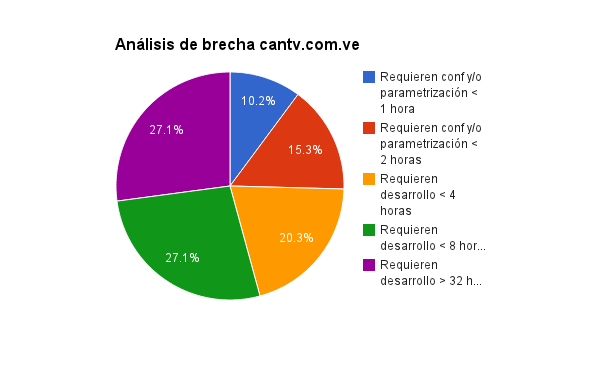
\includegraphics[width=.9\linewidth]{./images/graph_brecha_cantv_com_ve.png}
    \caption{Análisis de brecha portal cantv.com.ve}
    \end{figure}
\clearpage
\section{Cantidad de funcionalidades cubiertas por características de Plone}
\label{sec-3-2}



\includegraphics[width=.9\linewidth]{images/gap_plone_features_cantv_com_ve_34697d8c29178adac1ac2af1b6ca708d92074897.png}

\end{document}
